\documentclass{report}
\usepackage{amsmath}
\usepackage{amssymb}
\usepackage{hyperref,tikz}
\usepackage[margin=1in]{geometry}
\setlength{\parindent}{0pt}

\begin{document}
\thispagestyle{empty}
\begin{center} \LARGE Assignment 5 \end{center}

\section*{Part 1: Mathematical Derivations}

\subsection*{Q1. Building a decision tree by hand}
(a)

the entropy is \begin{equation}
    -\left( \frac{3}{10} \log_2(\frac{3}{10}) + \frac{7}{10} \log_2(\frac{7}{10}) \right)@ \approx 0.881290899231
\end{equation}

(b)



\begin{equation}\begin{split}
        H(S_{young}) &= 1\\
        H(S_{middle}) &= 0\\
        H(S_{senior}) &= -\left( \frac{1}{4} \log_2(\frac{1}{4}  ) + \frac{3}{4} \log_2(\frac{3}{4})  \right)=  0.81128
\end{split}
\end{equation}

\begin{equation}\begin{split}
        IG(S,Age) &= H(S) - \frac{S_{young}}{S} H(S_{young}) - \frac{S_{middle}}{S} H(S_{middle}) - \frac{S_{senior}}{S} H(S_{senior}) \\
        &\approx 0.881290899231 - (\frac{4}{10}   ) - \frac{4}{10} \cdot 0.88128\\
        &\approx 0.156770899
\end{split}
\end{equation}


\begin{equation}\begin{split}
    H(S_{High}) &= -\left(\frac{1}{3}\log_2(\frac{1}{3}) + \frac{2}{3}\log_2(\frac{2}{3})\right) \approx 0.9183\\
    H(S_{Medium}) &\approx 0.9183\\
    H(S_{Low}) &\approx 0.81128
\end{split}
\end{equation}

\begin{equation}
    IG(S,Income)=0.8813-\frac{3}{10}(0.9183) - \frac{3}{10}(0.9183) - \frac{4}{10}(0.81128) = 0.0058
\end{equation}

\begin{equation}
    \begin{split}
        H(S_{\not student}) &= -\left( \frac{2}{5}\log_2(\frac{2}{5}) + \frac{3}{5}\log_2(\frac{3}{5})  \right)= 0.97\\
        H(S_{ student}) &= 0 
    \end{split}
\end{equation}

\begin{equation}
    IG(S,Student)=0.8813-\frac{5}{10}(0.9710) = 0.3958
\end{equation}

the best root splitting feature is student because it provides the most information gain.

(c)

the "student" branch becomes pure. the "not student" branch remains impure. 

\begin{equation}
    H(S|Student) = -\left( \frac{2}{5}\log_2(\frac{2}{5})  + \frac{3}{5}\log_2(\frac{3}{5})  \right) = 0.971
\end{equation}

\begin{equation}
    IG(S,Age | Student) = 0.4
\end{equation}
the only branch where \(H(S_{age|student})\) is nonzero is when the age is senior which has a \(2/5\) probability and an entropy of 1.

\begin{equation}
    IG(S,Income | Student) = 2/5+2/5 = .8
\end{equation}

note
\begin{equation}\begin{split}
        H(S,High|student) &= 1\\
        H(S,Medium|student) &= 1\\
\end{split}
\end{equation}

the second best to split on is Age. 

(d)

\begin{figure}[!ht]
\centering
\resizebox{0.7\textwidth}{!}{%
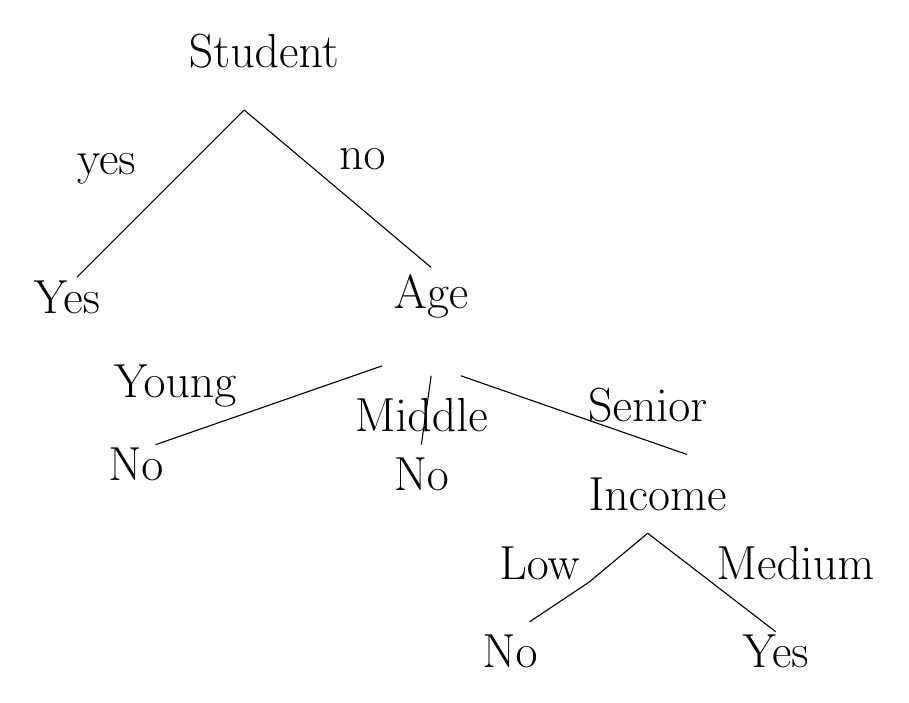
\begin{tikzpicture}
\tikzstyle{every node}=[font=\fontsize{18.2pt}{23.7pt}\selectfont]
\node [font=\fontsize{18.2pt}{23.7pt}\selectfont, inner xsep=0.080cm, inner ysep=0.085cm, rounded corners=0.020cm] at (11.5,14.25) {Student};
\draw [] (11.25,13.5) -- (9.125,11.375);
\draw [] (11.25,13.5) -- (13.625,11.5);
\node [font=\fontsize{18.2pt}{23.7pt}\selectfont, inner xsep=0.080cm, inner ysep=0.085cm, rounded corners=0.020cm] at (9.5,12.75) {yes};
\node [font=\fontsize{18.2pt}{23.7pt}\selectfont, inner xsep=0.080cm, inner ysep=0.085cm, rounded corners=0.020cm] at (12.75,12.875) {no};
\node [font=\fontsize{18.2pt}{23.7pt}\selectfont, inner xsep=0.080cm, inner ysep=0.085cm, rounded corners=0.020cm] at (13.625,11.125) {Age};
\draw [] (13,10.25) -- (10.125,9.25);
\draw [] (13.625,10.125) -- (13.5,9.25);
\draw [] (14,10.125) -- (16.875,9.125);
\node [font=\fontsize{18.2pt}{23.7pt}\selectfont, inner xsep=0.080cm, inner ysep=0.085cm, rounded corners=0.020cm] at (10.375,10) {Young};
\node [font=\fontsize{18.2pt}{23.7pt}\selectfont, inner xsep=0.080cm, inner ysep=0.085cm, rounded corners=0.020cm] at (13.5,9.625) {Middle};
\node [font=\fontsize{18.2pt}{23.7pt}\selectfont, inner xsep=0.080cm, inner ysep=0.085cm, rounded corners=0.020cm] at (16.375,9.75) {Senior};
\draw [] (16.375,8.125) -- (15.625,7.5);
\draw [] (15.625,7.5) -- (14.875,7);
\draw [] (16.375,8.125) -- (18,6.875);
\node [font=\fontsize{18.2pt}{23.7pt}\selectfont, inner xsep=0.080cm, inner ysep=0.085cm, rounded corners=0.020cm] at (16.5,8.625) {Income};
\node [font=\fontsize{18.2pt}{23.7pt}\selectfont, inner xsep=0.080cm, inner ysep=0.085cm, rounded corners=0.020cm] at (15,7.75) {Low};
\node [font=\fontsize{18.2pt}{23.7pt}\selectfont, inner xsep=0.080cm, inner ysep=0.085cm, rounded corners=0.020cm] at (18.25,7.75) {Medium};
\node [font=\fontsize{18.2pt}{23.7pt}\selectfont, inner xsep=0.080cm, inner ysep=0.085cm, rounded corners=0.020cm] at (9,11.125) {Yes};
\node [font=\fontsize{18.2pt}{23.7pt}\selectfont, inner xsep=0.080cm, inner ysep=0.085cm, rounded corners=0.020cm] at (9.875,9) {No};
\node [font=\fontsize{18.2pt}{23.7pt}\selectfont, inner xsep=0.080cm, inner ysep=0.085cm, rounded corners=0.020cm] at (13.5,8.875) {No};
\node [font=\fontsize{18.2pt}{23.7pt}\selectfont, inner xsep=0.080cm, inner ysep=0.085cm, rounded corners=0.020cm] at (14.625,6.625) {No};
\node [font=\fontsize{18.2pt}{23.7pt}\selectfont, inner xsep=0.080cm, inner ysep=0.085cm, rounded corners=0.020cm] at (18,6.625) {Yes};
\end{tikzpicture}
}%
\caption{Decision tree}
\label{fig:Decision_Tree}
\end{figure}




\subsection*{Q2. Information gain is always non-negative}
(a)

\begin{equation}
    \frac{d}{dx} \left( -\left( x\log_2(x) + (1-x)\log_2(1-x) \right) \right) = (\log_2(1-x) - \log_2(x))
\end{equation}

\begin{equation}
    \frac{d}{dx} \left( \log_2(1-x) - \log_2(x) \right)= -\frac{1}{x(1-x)\log(2)}
\end{equation}

for all \(x\in(0,1)\), this function is negative since \(x(1-x)\) is positive in this range. 


(b)
$$IG(S, A) = H(S) - H(S|A)$$
To prove $IG(S, A) \geq 0$, we must show $H(S) \geq H(S|A)$.

note
$$H(S) = -\sum_{c \in C} p_c \log_2(p_c)$$

since \(H\) is concave we can use Jensons on \(H\)

\begin{equation}\label{q2b}
    H\left( \sum_{v \in Values(A)} \frac{|S_v|}{|S|} P_v \right) \geq \sum_{v \in Values(A)} \frac{|S_v|}{|S|} H(P_v)
\end{equation}

the left side of eq~\ref{q2b} is just \(H(S)\) and the RHS is the conditional entropy \(H(S|A)\)

(c)

the information gain is 0 when a new piece of information does not help us differentiate the target value. the information gain is 1 (maximized) when the information lets us determine the target value exactly. 

imagine i have 10 numbers, first 5 are yes second 5 are no. 

if I receive the information about even or odd, it gives 0 information. if i receive information about greater than or less than 5, then I gain information of 1. 

\subsection*{Q3. Decision trees with continuous features}
(a)

we only need to tell when the label changes. the thresholds are 20, 30, 35, 40

(b)

$$H(S) = -\left(\frac{3}{6}\log_2\frac{3}{6} + \frac{3}{6}\log_2\frac{3}{6}\right) = 1.0 \text{ bit}$$

\begin{equation}\begin{split}
        IG(S,20) &= \frac{1}{6}(0) + \frac{5}{6}H(\frac{3}{5}, \frac{2}{5}) \approx  1 - 0.809 \approx 0.191\\
        IG(S,30) &= \frac{3}{6}H(\frac{2}{3}, \frac{1}{3}) + \frac{3}{6}H(\frac{1}{3}, \frac{2}{3}) \approx 1 - 0.918 \approx  0.082\\
        IG(S,35) &=\frac{4}{6}H(\frac{2}{4}, \frac{2}{4}) + \frac{2}{6}H(\frac{1}{2}, \frac{1}{2}) = 0\\
        IG(S,40) &=\frac{5}{6}H(\frac{3}{5}, \frac{2}{5}) + \frac{1}{6}(0)\approx 1 - 0.809 \approx 0.191
\end{split}
\end{equation}

either 20 or 40 both work with an information gain of approximately \(0.191\)

(c)

the threshold 35 did not yield any information gain. 

the left and the right of 35 remained a 5050 split and so the information received from knowing the distribution greater than or less than 35 yielded no infromation gain. 

\section*{Reflection + Statistics Section}
(a)

(b) 

(c) 

(d) Total: \\

Part 1: \\
Q1: \\

Part 2: \\
Q1: 20 min, Q2: \\

Part 3: \\
Q1: \\

(e)


\end{document}
